\newcommand{\mpsspin}{
	
\begin{tikzpicture}
		% filled circle with thick black outline (center fixed at origin)
		\node[draw=black, thick, circle, minimum size=.3cm, inner sep=0pt, fill=\maincolor] (c) at (0,0) {};

	\end{tikzpicture}
}
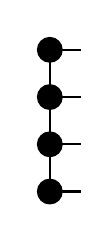
\begin{tikzpicture}
	\def\spindist{.6cm}
	\def\spinout{.4cm}
	% Declare layers
	\pgfdeclarelayer{background}
	\pgfsetlayers{background,main}

	% Spins
	\node (spin1) at (0, 0) {\mpsspin};
	\node (spin2) at ([yshift=-\spindist]spin1) {\mpsspin};
	\node (spin3) at ([yshift=-\spindist]spin2) {\mpsspin};
	\node (spin4) at ([yshift=-\spindist]spin3) {\mpsspin};

	% Line in the background layer
	\begin{pgfonlayer}{background}
		% connection between spins
		\draw[thick] (spin1.center) -- (spin4.center);

		% spin to out
		\draw[thick] (spin1.center) -- ([xshift=\spinout]spin1.center);
		\draw[thick] (spin2.center) -- ([xshift=\spinout]spin2.center);
		\draw[thick] (spin3.center) -- ([xshift=\spinout]spin3.center);
		\draw[thick] (spin4.center) -- ([xshift=\spinout]spin4.center);
	\end{pgfonlayer}
\end{tikzpicture}